%%%%%%%%%%%%%%%%%%%%%%%%%%%%%%%%%%%%%%%%%%%%%%%%%%%%%%%%%%%%%%%%%%%%%%%%%%%%%%%%%%%%%%%%%%%%%%%%%%
%% This file contains a description of the UI and functionality for the editor portion of the GUI.
%% Trevor Morse
%% CS 383
%% 10/31/2016
%%%%%%%%%%%%%%%%%%%%%%%%%%%%%%%%%%%%%%%%%%%%%%%%%%%%%%%%%%%%%%%%%%%%%%%%%%%%%%%%%%%%%%%%%%%%%%%%%%

\documentclass{article}

\begin{document}
	\section{Editor}
	The editor is that part of the main window in which the frames and the frames' LED cells are displayed.  This editor window seeks to keep all the old functionality while adding improvements, such as an easier process for adding and deleting frames, and different navigational  processes.
	\subsection{Mock-up}
	\begin{figure}[!htb]
		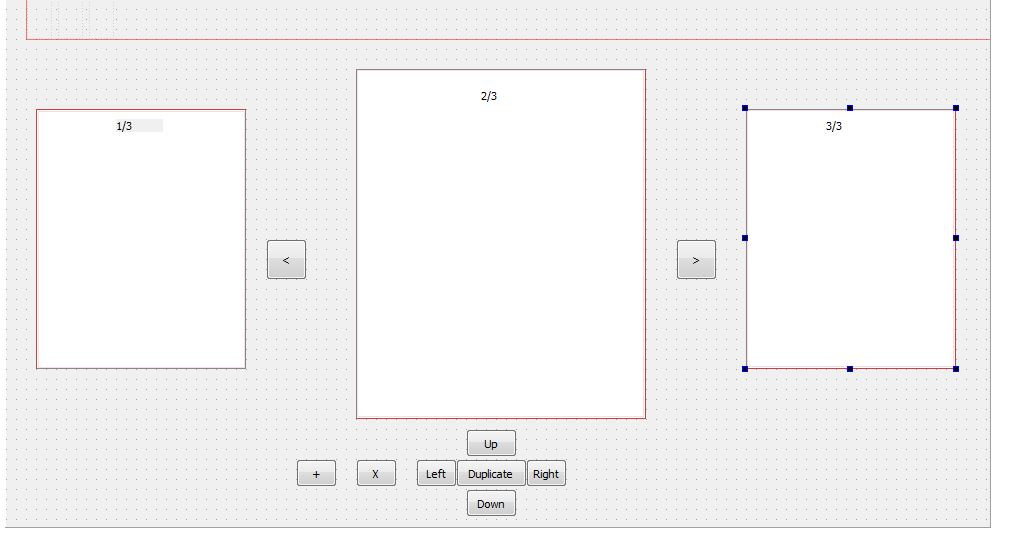
\includegraphics[width=\linewidth]{/Users/Zachary/tol/docs/design_spec/current_iteration_editor.jpg}
		\caption{Initial Mock-up of the editor section of the GUI.}
		\label{fig:editor_view}
	\end{figure}
	
	\subsection{Functionality}
	The following descriptions reference Figure \ref{fig:editor_view} above.
	\begin{itemize}
		\item This section of the GUI is the primary area for editing a frame within the overall animation. The primary focus is on the current frame in the center of the view, with smaller references to the previous and subsequent frames to the sides.  The premise behind this design choice is that with three visible frames in the main editing window, the user will be able to more easily craft animations that require multiple frames, such as doing a "w".  The user, with three immediately visible frames, will be able to view duplications and shifts more easily.
		\item Navigation:
		\begin{itemize}
			\item Above the current frame, there is an indicator of the current position relative to the total number of frames, allowing the user a better idea as to where each frame is in the animation.
			\item In order to navigate to a previous or subsequent slide, the user will click on the arrows to the sides of the current frame.  When one of these buttons is clicked, then it will shift the frames left or right, modifying the current view.  This creates a rotating list of frames for the user.
			\item Possible Addition: Mini-frame representations surrounding the numbers indicating the position of the frame. These could allow for speedy navigation across a large number of frames.  Essentially a list of thumbnails, this allows the user to click to the area of the animation as needed, rather than rotating all the way through with the left/right navigation buttons.
		\end{itemize}
		\item Editing:
		\begin{itemize}
			\item In order to edit a given frame, the user will utilize a combination of features in this section as well as in the toolboxes. (See Section \ref{toolbox} for more details.)
			\item The current frame will be enlarged in the center of the view. Each panel inside represents an LED panel on the tower (panels in the figure are not necessarily to scale).  The panels are also only editable when in the current frame.  If in the previous or next frame, the user will be unable to edit them, preventing any slips on already finished or yet to be edited frames.  This also allows the user to focus on the current frame.
			\item The user will be able to select one or more LED panels at a time and specify the given options within the toolboxes.
			\item Below the current frame are a series of buttons. One allows the user to insert a new, blank frame immediately after the current frame. Another button allows the user to duplicate the current frame in a new frame after it.  The button with an "x" on it deletes the current frame.  The up/down/left/right labeled buttons are for the shifted duplications as used in the original tower lights animator.  Thus, maintaining the old functionality alongside new additions. 
		\end{itemize}
	\end{itemize}
	
	\subsection{Notes}
	\begin{itemize}
		\item The editor section of the GUI  works alongside the toolboxes. These toolboxes willl display to the left of the editor. They will provide options for editing a particular LED panel and/or overall frame. %TODO: reference the Toolbox section here
		\item There will also be options in the GUI's menus that will help with more efficient editing and navigation of frames.
		\item The development of the UI of the editor was one of the first to-do items determined by the team.  This was to help solidify the design before construction of the code itself. Once the design was solidified, more in-depth functionality was added.  This included working navigation, adding and deleting frames, etc.
	\end{itemize}
	
\end{document}